%%%%%%%%%%%%%%%%%%%%%%%%%%%%%%%%%%%%%%%%%%%%%%%%%%%%%%%%%%%%%%%%%%%%%%%%%%%%%%%%
% Tutorial slides on Python.
%
% Author: Prabhu Ramachandran <prabhu at aero.iitb.ac.in>
% Copyright (c) 2005-2008, Prabhu Ramachandran
%%%%%%%%%%%%%%%%%%%%%%%%%%%%%%%%%%%%%%%%%%%%%%%%%%%%%%%%%%%%%%%%%%%%%%%%%%%%%%%%

\documentclass[14pt,compress]{beamer}
%\documentclass[draft]{beamer}
%\documentclass[compress,handout]{beamer}
%\usepackage{pgfpages} 
%\pgfpagesuselayout{2 on 1}[a4paper,border shrink=5mm]

% Modified from: generic-ornate-15min-45min.de.tex
\mode<presentation>
{
  \usetheme{Warsaw}
  \useoutertheme{split}
  \setbeamercovered{transparent}
}

\usepackage[english]{babel}
\usepackage[latin1]{inputenc}
%\usepackage{times}
\usepackage[T1]{fontenc}

% Taken from Fernando's slides.
\usepackage{ae,aecompl}
\usepackage{mathpazo,courier,euler}
\usepackage[scaled=.95]{helvet}

\definecolor{darkgreen}{rgb}{0,0.5,0}

\usepackage{listings}
\lstset{language=Python,
    basicstyle=\ttfamily\bfseries,
    commentstyle=\color{red}\itshape,
  stringstyle=\color{darkgreen},
  showstringspaces=false,
  keywordstyle=\color{blue}\bfseries}

%%%%%%%%%%%%%%%%%%%%%%%%%%%%%%%%%%%%%%%%%%%%%%%%%%%%%%%%%%%%%%%%%%%%%%
% Macros
\setbeamercolor{emphbar}{bg=blue!20, fg=black}
\newcommand{\emphbar}[1]
{\begin{beamercolorbox}[rounded=true]{emphbar} 
      {#1}
 \end{beamercolorbox}
}
\newcounter{time}
\setcounter{time}{0}
\newcommand{\inctime}[1]{\addtocounter{time}{#1}{\tiny \thetime\ m}}

\newcommand{\typ}[1]{\texttt{#1}}

\newcommand{\kwrd}[1]{ \texttt{\textbf{\color{blue}{#1}}}  }

%%% This is from Fernando's setup.
% \usepackage{color}
% \definecolor{orange}{cmyk}{0,0.4,0.8,0.2}
% % Use and configure listings package for nicely formatted code
% \usepackage{listings}
% \lstset{
%    language=Python,
%    basicstyle=\small\ttfamily,
%    commentstyle=\ttfamily\color{blue},
%    stringstyle=\ttfamily\color{orange},
%    showstringspaces=false,
%    breaklines=true,
%    postbreak = \space\dots
% }


%%%%%%%%%%%%%%%%%%%%%%%%%%%%%%%%%%%%%%%%%%%%%%%%%%%%%%%%%%%%%%%%%%%%%%
% Title page
\title[Basic Python]{Python,\\a great programming toolkit:\\
numerics and plotting}

\author[Asokan \& Prabhu] {Asokan Pichai\\Prabhu Ramachandran}

\institute[IIT Bombay] {Department of Aerospace Engineering\\IIT Bombay}
\date[] {26, July 2009}
%%%%%%%%%%%%%%%%%%%%%%%%%%%%%%%%%%%%%%%%%%%%%%%%%%%%%%%%%%%%%%%%%%%%%%

%\pgfdeclareimage[height=0.75cm]{iitmlogo}{iitmlogo}
%\logo{\pgfuseimage{iitmlogo}}


%% Delete this, if you do not want the table of contents to pop up at
%% the beginning of each subsection:
\AtBeginSubsection[]
{
  \begin{frame}<beamer>
    \frametitle{Outline}
    \tableofcontents[currentsection,currentsubsection]
  \end{frame}
}

\AtBeginSection[]
{
  \begin{frame}<beamer>
    \frametitle{Outline}
    \tableofcontents[currentsection,currentsubsection]
  \end{frame}
}

% If you wish to uncover everything in a step-wise fashion, uncomment
% the following command: 
%\beamerdefaultoverlayspecification{<+->}

%\includeonlyframes{current,current1,current2,current3,current4,current5,current6}

%%%%%%%%%%%%%%%%%%%%%%%%%%%%%%%%%%%%%%%%%%%%%%%%%%%%%%%%%%%%%%%%%%%%%%
% DOCUMENT STARTS
\begin{document}

\begin{frame}
  \titlepage
\end{frame}
\begin{frame}
  {Acknowledgements}
  \begin{center}
  This program is conducted by\\
  IIT, Bombay\\
  through CDEEP\\
  as part of  the open source initiatives\\
  under the aegis of\\
  \alert{National Mission on Education through ICT,} \\
  Ministry of HRD.
  \end{center}
\end{frame}

\begin{frame}
  \frametitle{Outline}
  \tableofcontents
  % You might wish to add the option [pausesections]
\end{frame}

\begin{frame}{Goal of the Workshop}

        At the end of this program, successful participants will be able
        to use python as their scripting and problem solving language.
        Aimed at Engg. students--focus on basic numerics and plotting--
        but should serve a similar purpose for others.\\

        At the minimum you will be able to use Python for your plotting immediately.

\end{frame}

\begin{frame}{Checklist}
    
  \begin{description}
	\item[pylab] matplotlib interface 
	\item[numpy] Array computing
        \item[scipy] numerical work
        \item[mayavi] \typ{enthought.mayavi}: 3D viz.
  \end{description}
\end{frame}

\section{30000 feet view}
\begin{frame}{Lets see what we can do!}
  \huge
  Hold on to your seatbelts
\end{frame}

\begin{frame}
  {That was done by\ldots}
  \begin{description}[CalisthenicsIsAnArt]
      \item[Arrays] 2--3 lines; 5 minutes to learn
      \item[2D plots] 5 lines; 10 minutes to learn
      \item[Simple 3D plots] 5 lines; 10 minutes to learn; GUI
          exploration!
      \item[Complex plots] relatively short (10-15 lines); more time to master; 
  \end{description}
  \inctime{15}
\end{frame}

\section{Matplotlib}

\subsection{Basic \typ{numpy} }

\newcommand{\num}{\texttt{numpy}}

\begin{frame}
  \frametitle{The \num\ module}
  \begin{itemize}
      \item Why?
  \item What:
    \begin{itemize}
    \item An efficient and powerful array type for various common data
      types
    \item Abstracts out the most commonly used standard operations on
      arrays
    \end{itemize}
  \end{itemize}
\end{frame}

\begin{frame}[fragile]
  \frametitle{Examples of \num}
\begin{lstlisting}
# Simple array math example
>>> from numpy import *
>>> a = array([1,2,3,4])
>>> b = array([2,3,4,5])
>>> a*2 + b + 1 # Basic math!
array([5, 8, 11, 14])
# Pi and e are defined.
>>> x = linspace(0.0, 10.0, 1000)
>>> x *= 2*pi/10 # inplace.
# apply functions to array.
>>> y = sin(x)
\end{lstlisting}
\end{frame}

\begin{frame}
  \frametitle{Basic concepts}
  \begin{itemize}
  \item fixed size (\typ{arr.size});
  \item Same type (\typ{arr.dtype}) of data
  \item arbitrary dimensionality
  \item \typ{arr.shape}: size in each dimension
  \item \alert{Note:} \typ{len(arr) != arr.size} in general
  \item \alert{Note:} By default array operations are performed
    \alert{elementwise}
  \item Indices, slicing: just like lists 
  \end{itemize}
\end{frame}


\begin{frame}[fragile]
  \frametitle{More examples of \num}
\vspace*{-8pt}
\begin{lstlisting}
>>> x = array([1., 2, 3, 4])
>>> size(x)
4
>>> x.dtype # What is a.dtype?
dtype('float64')
>>> x.shape
(4,)
>>> print rank(x), x.itemsize
1 8
>>> x[0] = 10
>>> print x[0], x[-1]
10.0 4.0
\end{lstlisting}
    
\inctime{10}
\end{frame}



%%%%%%%%%%%%%%%%%%%%%%%%%%%%%%%%%%%%%%%%%%%%%%%%%%%%%%%%%%%%%%%%%%%%%%
\subsection{Plotting with \typ{pylab}}

\begin{frame}
    {IPython's \typ{pylab} mode}
\begin{itemize}
    \item \typ{pylab}: convenient 2D plotting interface to MPL
    \item Immediate use: \typ{ipython -pylab}
    \item Imports all of pylab for you!
    \item Allows for interactive plotting
\end{itemize}
\end{frame}

\begin{frame}[fragile]
    \frametitle{Basic 2D plotting}

\begin{lstlisting}
>>> x = linspace(0, 2*pi, 1000)
>>> plot(x, sin(x)) 
>>> plot(x, sin(x), 'ro')
>>> xlabel(r'$\chi$', color='g')
# LaTeX markup!
>>> ylabel(r'sin($\chi$)', color='r')
>>> title('Simple figure', fontsize=20)
>>> savefig('/tmp/test.eps')
\end{lstlisting}
\begin{itemize}
  \item Also: PNG, PDF, PS, EPS, SVG, PDF
\end{itemize}
\end{frame}
       

\begin{frame}[fragile]
  \frametitle{Basic plotting \ldots}
\begin{lstlisting}
# Set properties of objects:
>>> l, = plot(x, sin(x))
# Why "l,"?
>>> setp(l, linewidth=2.0, color='r')
>>> l.set_linewidth(2.0)
>>> draw() # Redraw.
>>> setp(l) # Print properties
>>> clf() # Clear figure.
>>> close() # Close figure.
\end{lstlisting}
\end{frame}

\begin{frame}[fragile]
    \frametitle{Multiple figures}

\begin{lstlisting}
>>> figure(1)
>>> plot(x, sin(x))
>>> figure(2)
>>> plot(x, tanh(x))
>>> figure(1)
>>> title('Easy as 1,2,3')
\end{lstlisting}
    
\end{frame}


\begin{frame}[fragile]
  \frametitle{Legends and Annotation}
\begin{lstlisting}
>>> plot(x, cos(5*x), 'r--', 
         label='cosine')
>>> plot(x, sin(5*x), 'g--', 
         label='sine')
>>> legend() 
# Or use:
>>> legend(['cosine', 'sine'])
# Annotation:
>>> text(1,0, '(1,0)')
\end{lstlisting}
\end{frame}

\begin{frame}[fragile]
    \frametitle{More commands \ldots}
    \begin{lstlisting}
# semilog, loglog 
>>> x = 10.**(-arange(100)*0.1)
>>> semilogx(x, x)
>>> semilogy(x, x)
>>> loglog(x, x)
>>> loglog(x, x*x)
    \end{lstlisting}
\end{frame}

\begin{frame}[fragile]
    \frametitle{More plots \ldots}
    \begin{lstlisting}
>>> clf()
>>> t = arange(0.1, 4, 0.1)
>>> s = exp(-t)
>>> e = 0.1*abs(randn(len(s)))
>>> errorbar(t, s, e)
# Scatter plots
>>> clf()
>>> t = randn(len(e))
>>> scatter(t, e, c=s)
    \end{lstlisting}
\end{frame}

\begin{frame}[fragile]
    \frametitle{Note: \typ{pylab} in Python scripts}
\begin{lstlisting}
import pylab
x = pylab.linspace(0, 20, 1000)
pylab.plot(x, pylab.sin(x))

# Can also use:
from pylab import linspace, sin, plot
\end{lstlisting}
\end{frame}

%%%%%%%%%%%%%%%%%%%%%%%%%%%%%%%%%%%%%%%%%%%%%%%%%%%%%%%%%%%%%%%%%%%%%%

\begin{frame}[fragile]
  \frametitle{X-Y plot}
  \begin{columns}
    \column{0.5\textwidth}
    \hspace*{-0.5in}
    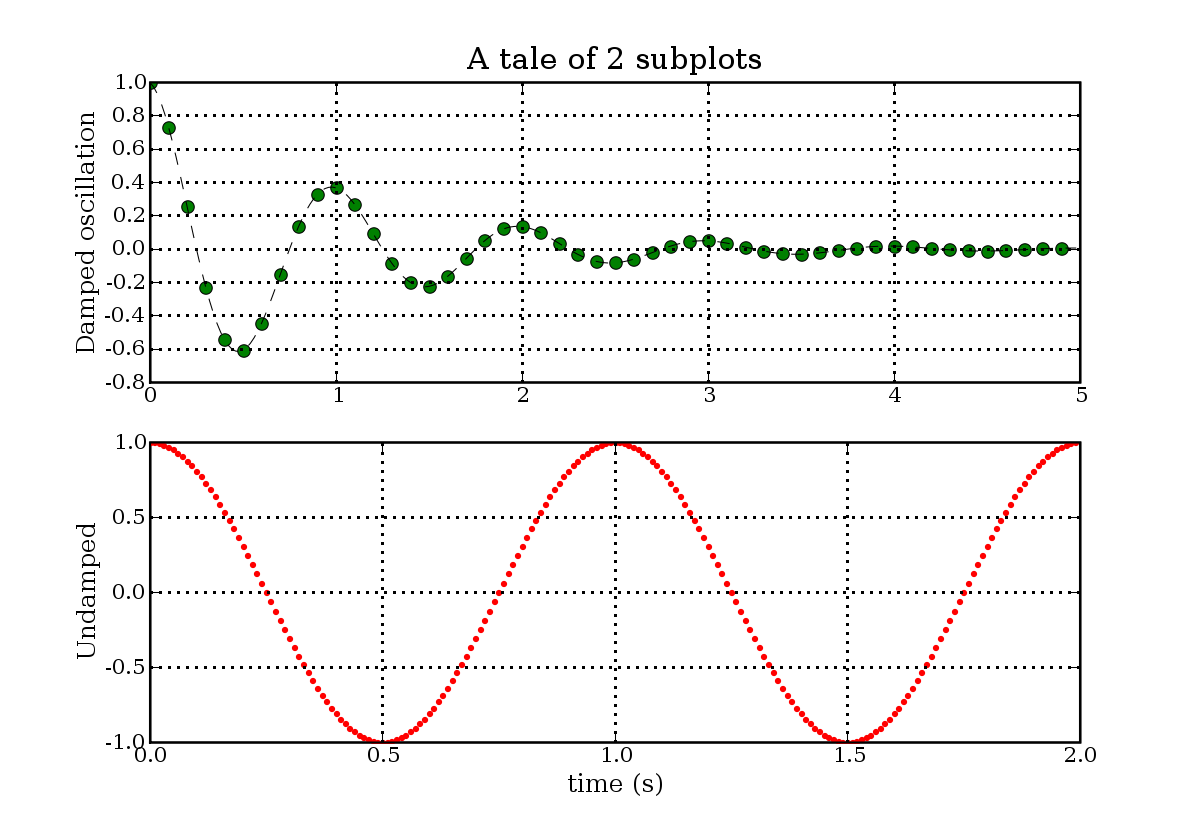
\includegraphics[height=2in, interpolate=true]{data/xyplot}
    \column{0.45\textwidth}
    \begin{block}{Example code}
    \tiny
\begin{lstlisting}
t1 = arange(0.0, 5.0, 0.1)
t2 = arange(0.0, 5.0, 0.02)
t3 = arange(0.0, 2.0, 0.01)
subplot(211)
plot(t1, cos(2*pi*t1)*exp(-t1), 'bo', 
     t2, cos(2*pi*t2)*exp(-t2), 'k')
grid(True)
title('A tale of 2 subplots')
ylabel('Damped')
subplot(212)
plot(t3, cos(2*pi*t3), 'r--')
grid(True)
xlabel('time (s)')
ylabel('Undamped')
\end{lstlisting}
    \end{block}
  \end{columns}
\end{frame}

\begin{frame}[fragile] \frametitle{Semi-log and log-log plots}
  \begin{columns}
    \column{0.5\textwidth}
    \hspace*{-0.5in}
  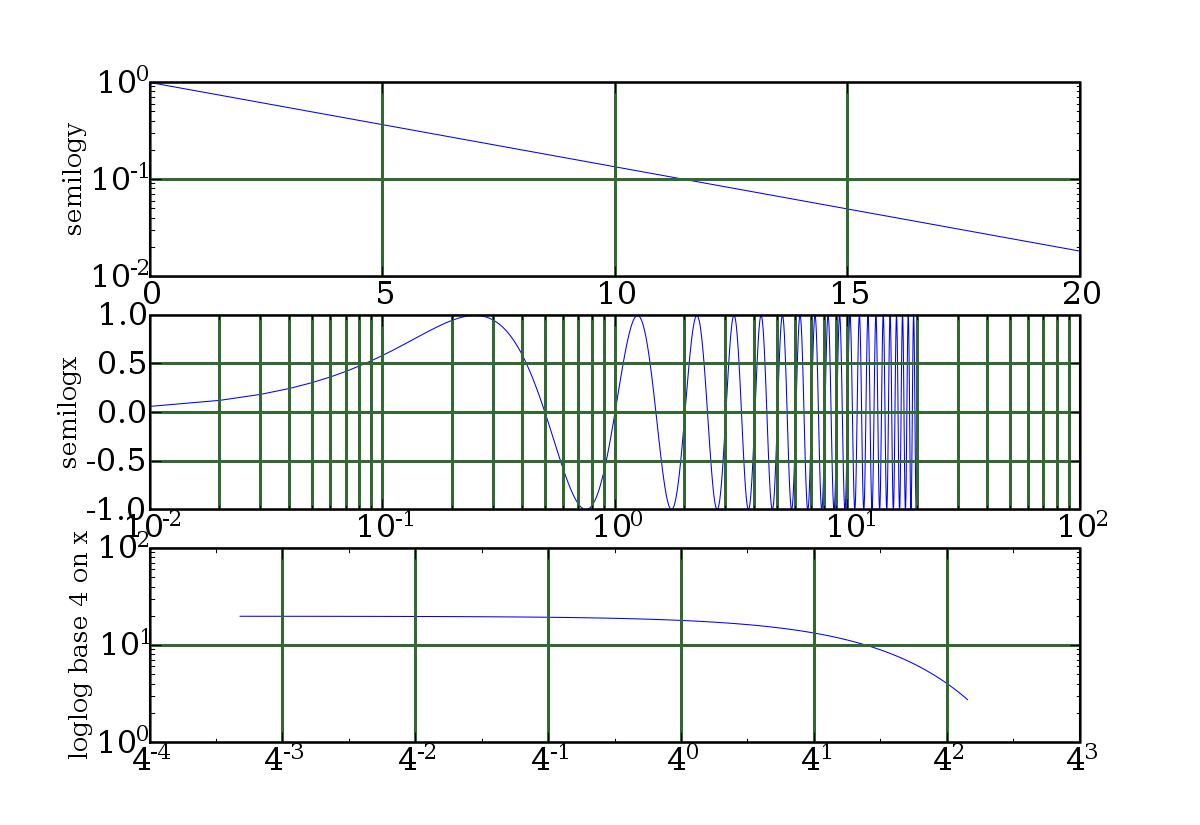
\includegraphics[height=2in, interpolate=true]{data/log}  
    \column{0.45\textwidth}
    \begin{block}{Example code}
    \tiny
\begin{lstlisting}
dt = 0.01
t = arange(dt, 20.0, dt)
subplot(311)
semilogy(t, exp(-t/5.0))
ylabel('semilogy')
grid(True)
subplot(312)
semilogx(t, sin(2*pi*t))
ylabel('semilogx')
grid(True)
# minor grid on too
gca().xaxis.grid(True, which='minor')  
subplot(313)
loglog(t, 20*exp(-t/10.0), basex=4)
grid(True)
ylabel('loglog base 4 on x')
\end{lstlisting}
  \end{block}
\end{columns}
\end{frame}

\begin{frame}[fragile] \frametitle{Errorbar}
  \begin{columns}
    \column{0.5\textwidth}
    \hspace*{-0.5in}
  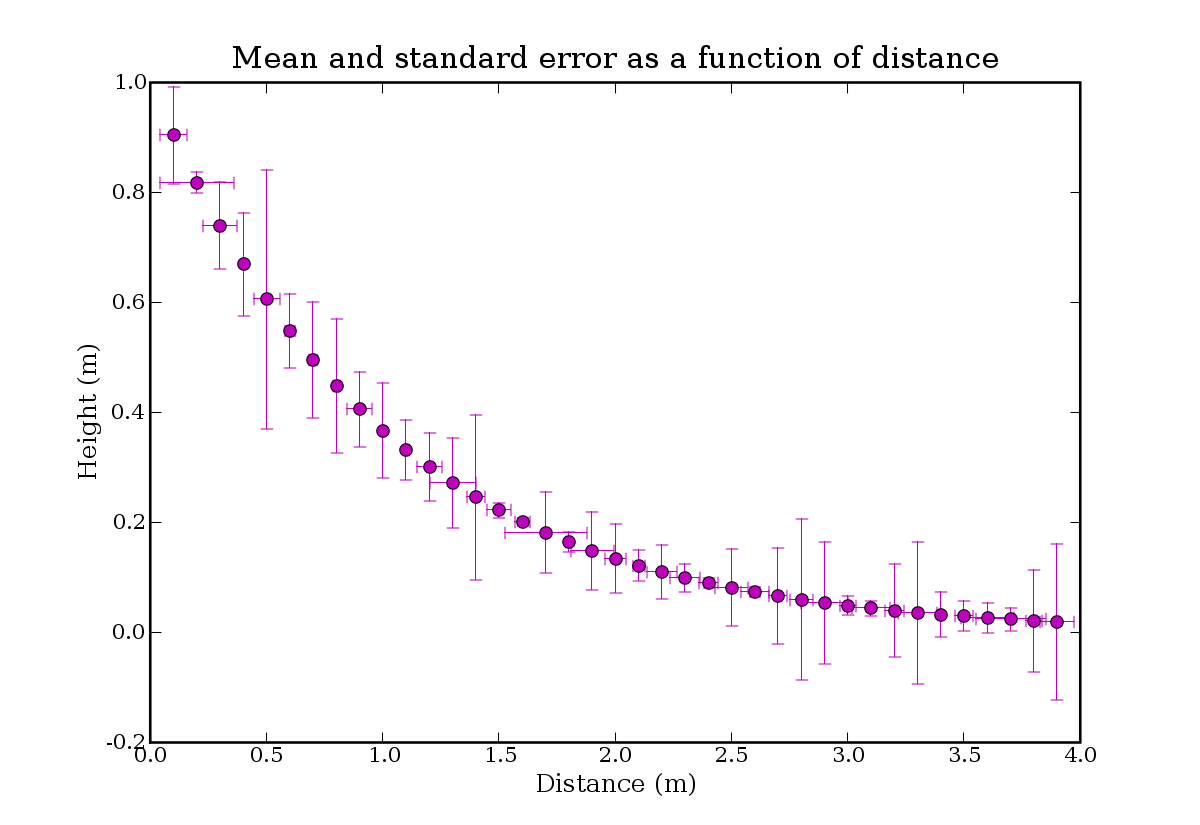
\includegraphics[height=2in, interpolate=true]{data/errorbar}  
    \column{0.45\textwidth}
    \begin{block}{Example code}
    \tiny
\begin{lstlisting}
t = arange(0.1, 4, 0.1)
s = exp(-t)
e = 0.1*abs(randn(len(s)))
f = 0.1*abs(randn(len(s)))
g = 2*e
h = 2*f
errorbar(t, s, [e,g], f, fmt='o')
xlabel('Distance (m)')
ylabel('Height (m)')
title('Mean and standard error '\
      'as a function of distance')
\end{lstlisting}
  \end{block}
\end{columns}
\end{frame}

\begin{frame}[fragile] \frametitle{Histogram}
  \begin{columns}
    \column{0.5\textwidth}
    \hspace*{-0.5in}
  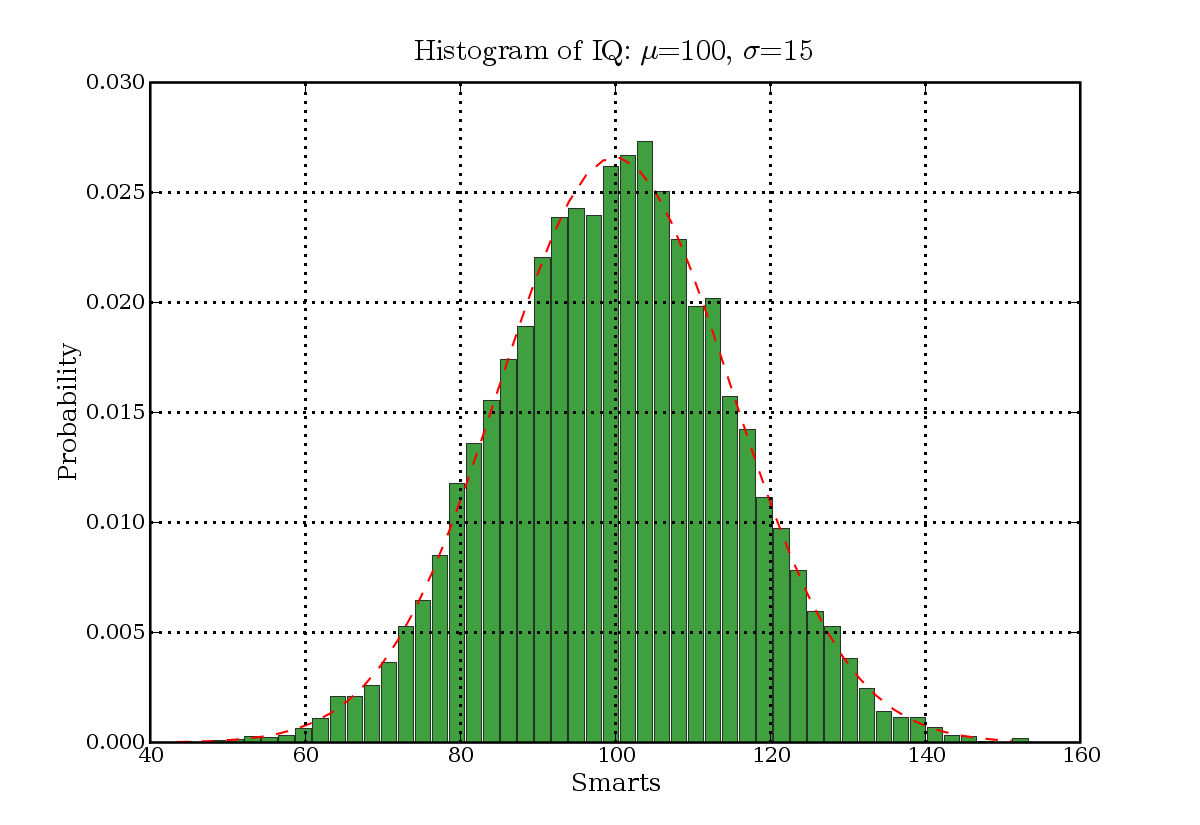
\includegraphics[height=2in, interpolate=true]{data/histogram}  
    \column{0.45\textwidth}
    \begin{block}{Example code}
    \tiny
\begin{lstlisting}
mu, sigma = 100, 15
x = mu + sigma*randn(10000)
# the histogram of the data
n, bins, patches = hist(x, 100, normed=1)
# add a 'best fit' line
y = normpdf( bins, mu, sigma)
l = plot(bins, y, 'r--', linewidth=2)
xlim(40, 160)
xlabel('Smarts')
ylabel('P')
title(r'$\rm{IQ:}\/ \mu=100,\/ \sigma=15$')
\end{lstlisting}
  \end{block}
\end{columns}
\end{frame}

\begin{frame}[fragile] \frametitle{Bar charts}
  \begin{columns}
    \column{0.5\textwidth}
    \hspace*{-0.5in}
  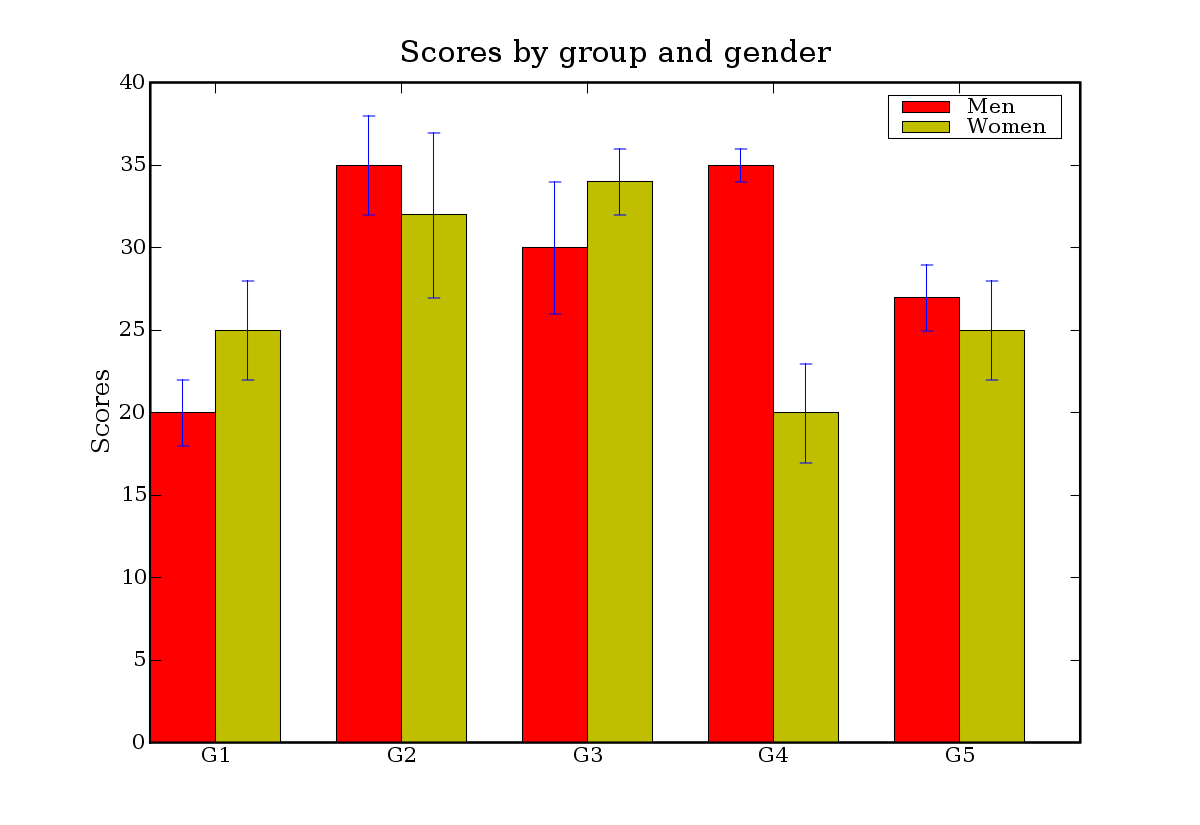
\includegraphics[height=2in, interpolate=true]{data/barchart}  
    \column{0.45\textwidth}
    \begin{block}{Example code}
    \tiny
\begin{lstlisting}
N = 5
menMeans = (20, 35, 30, 35, 27)
menStd =   ( 2,  3,  4,  1,  2)
# the x locations for the groups
ind = arange(N) 
# the width of the bars
width = 0.35       
p1 = bar(ind, menMeans, width, 
         color='r', yerr=menStd)
womenMeans = (25, 32, 34, 20, 25)
womenStd =   ( 3,  5,  2,  3,  3)
p2 = bar(ind+width, womenMeans, width, 
         color='y', yerr=womenStd)
ylabel('Scores')
title('Scores by group and gender')
xticks(ind+width, 
       ('G1', 'G2', 'G3', 'G4', 'G5'))
xlim(-width,len(ind))
yticks(arange(0,41,10))
legend((p1[0], p2[0]), 
       ('Men', 'Women'), shadow=True)
\end{lstlisting}
  \end{block}
\end{columns}
\end{frame}

\begin{frame}[fragile] \frametitle{Pie charts}
  \begin{columns}
    \column{0.5\textwidth}
    \hspace*{-0.4in}
  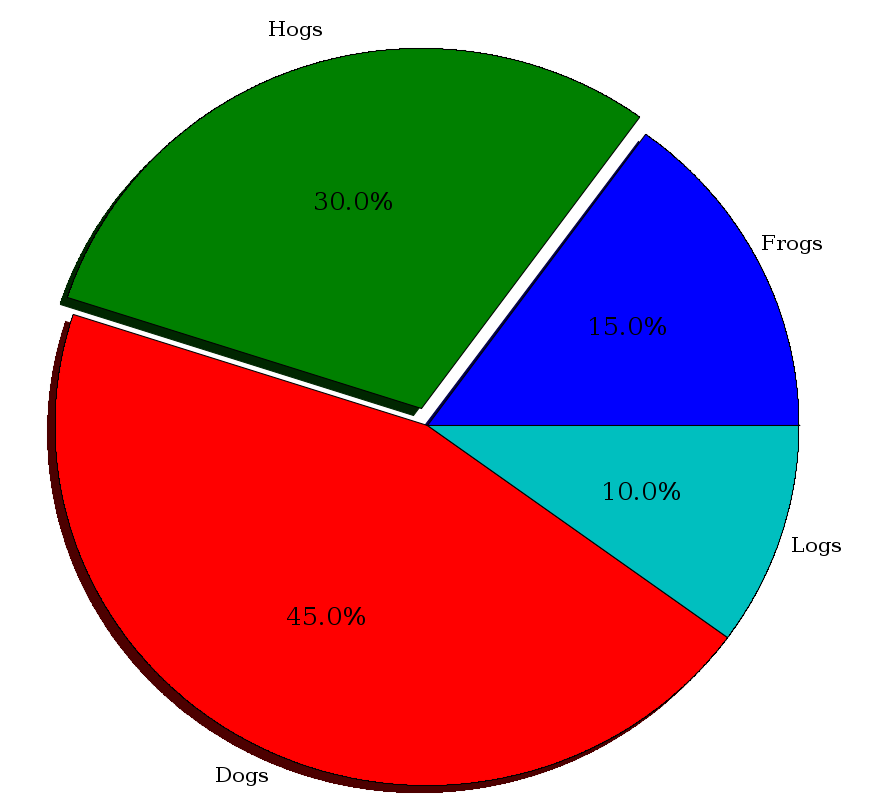
\includegraphics[height=2.0in, interpolate=true]{data/piechart}  
    \column{0.45\textwidth}
    \begin{block}{Example code}
    \tiny
\begin{lstlisting}
# make a square figure and axes
figure(1, figsize=(8,8))
ax = axes([0.1, 0.1, 0.8, 0.8])
labels = 'Frogs', 'Hogs', 'Dogs', 'Logs'
fracs = [15,30,45, 10]
explode=(0, 0.05, 0, 0)
pie(fracs, explode=explode, labels=labels, 
    autopct='%1.1f%%', shadow=True)
title('Raining Hogs and Dogs', 
      bbox={'facecolor':'0.8', 'pad':5})
\end{lstlisting}
  \end{block}
\end{columns}
\end{frame}

\begin{frame}[fragile] \frametitle{Scatter plots}
  \begin{columns}
    \column{0.5\textwidth}
    \hspace*{-0.4in}
  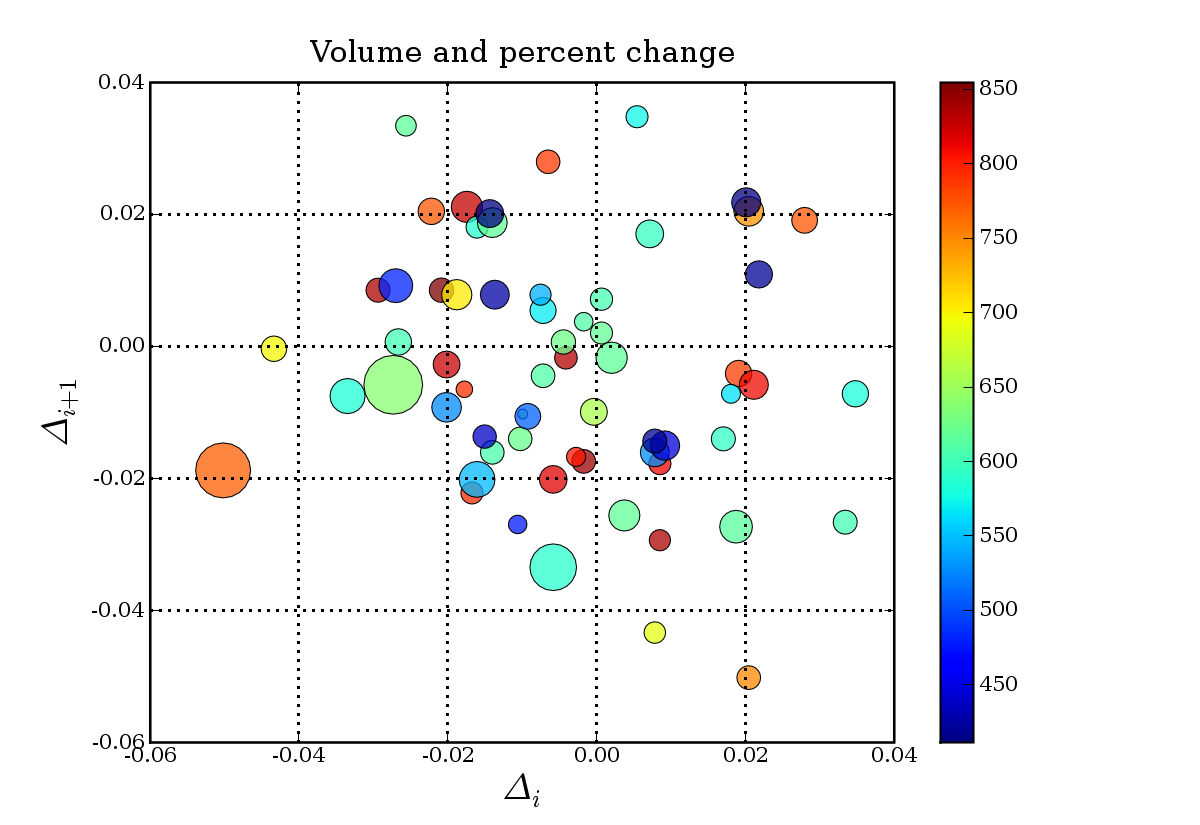
\includegraphics[height=2in, interpolate=true]{data/scatter}  
    \column{0.45\textwidth}
    \begin{block}{Example code}
    \tiny
\begin{lstlisting}
N = 30
x = 0.9*rand(N)
y = 0.9*rand(N)
# 0 to 10 point radiuses
area = pi*(10 * rand(N))**2 
volume = 400 + rand(N)*450
scatter(x,y,s=area, marker='o', c=volume, 
        alpha=0.75)
xlabel(r'$\Delta_i$', size='x-large')
ylabel(r'$\Delta_{i+1}$', size='x-large')
title(r'Volume and percent change')
grid(True)
colorbar()
savefig('scatter')
\end{lstlisting}
  \end{block}
\end{columns}
\end{frame}

\begin{frame}[fragile] \frametitle{Polar}
  \begin{columns}
    \column{0.5\textwidth}
    \hspace*{-0.5in}
  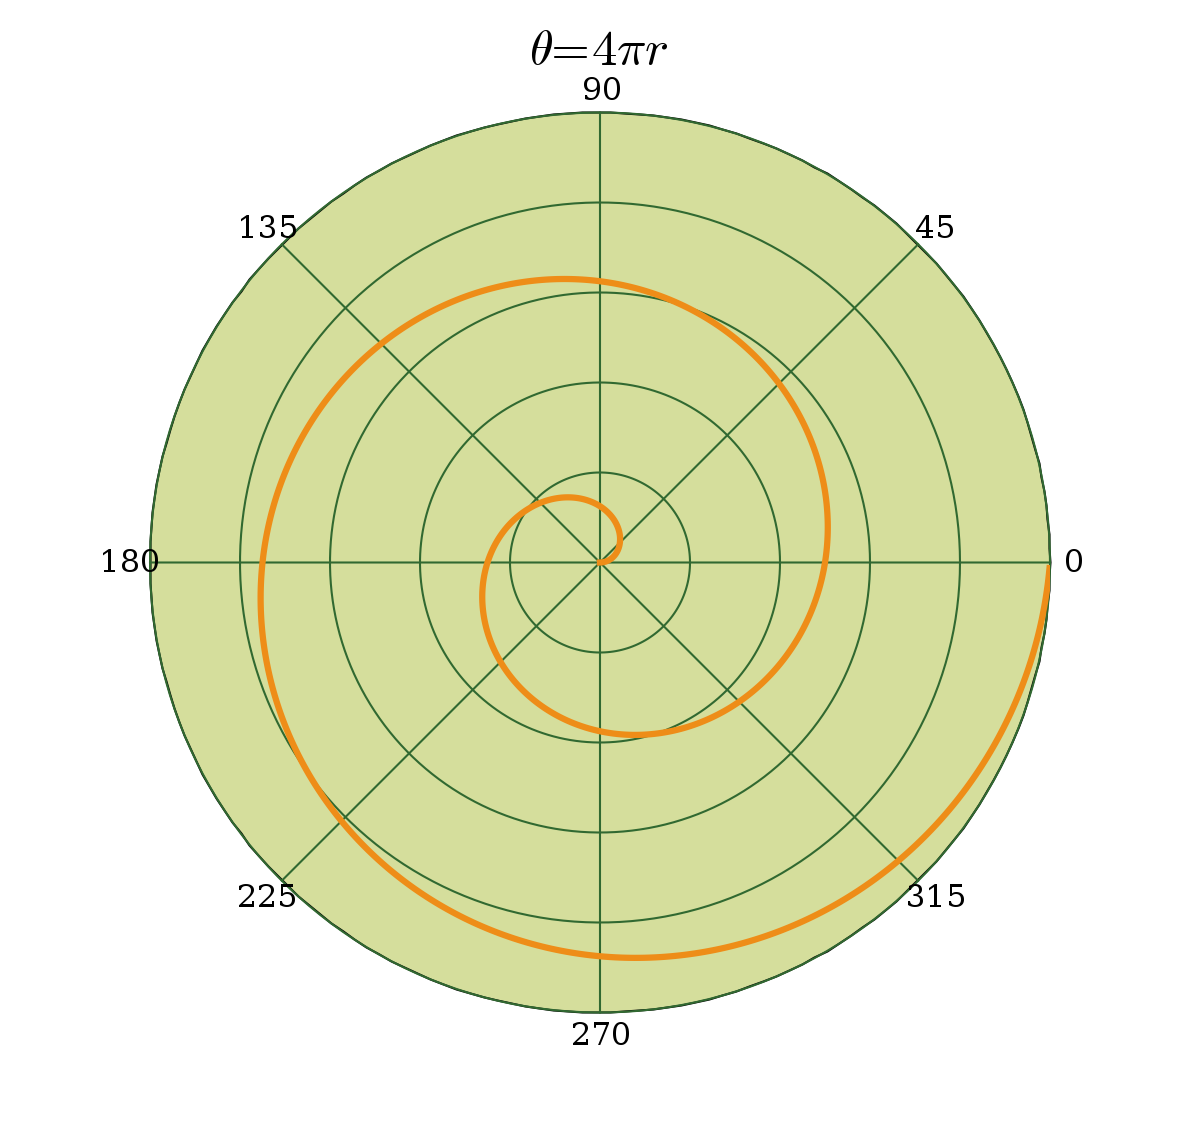
\includegraphics[height=2in, interpolate=true]{data/polar}  
    \column{0.45\textwidth}
    \begin{block}{Example code}
    \tiny
\begin{lstlisting}
figure(figsize=(8,8))
ax = axes([0.1, 0.1, 0.8, 0.8], 
          polar=True, 
          axisbg='#d5de9c')
r = arange(0,1,0.001)
theta = 2*2*pi*r
polar(theta, r, color='#ee8d18', lw=3)
# the radius of the grid labels
setp(ax.thetagridlabels, y=1.075) 
title(r"$\theta=4\pi r", fontsize=20)
\end{lstlisting}
  \end{block}
\end{columns}
\end{frame}

\begin{frame}[fragile] \frametitle{Contours}
  \begin{columns}
    \column{0.45\textwidth}
    \hspace*{-0.5in}
  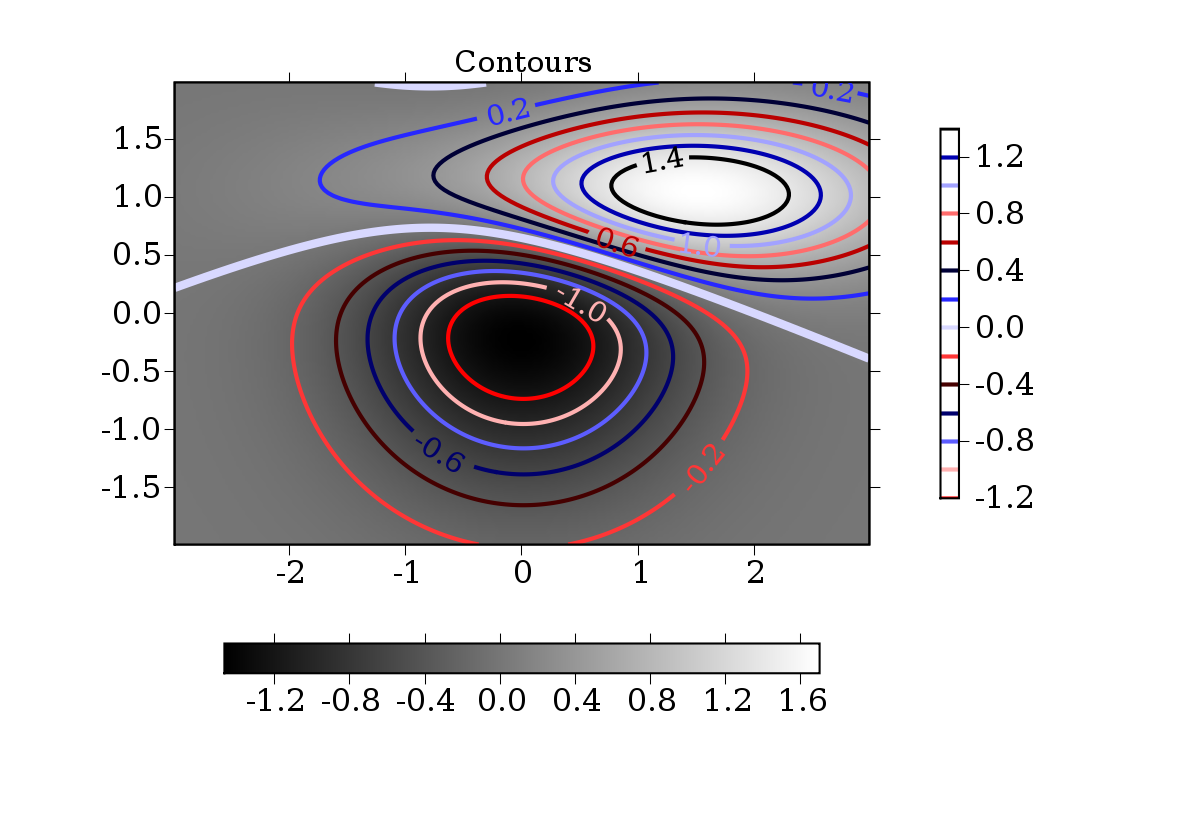
\includegraphics[height=2in, interpolate=true]{data/contour}  
    \column{0.525\textwidth}
    \begin{block}{Example code}
    \tiny
\begin{lstlisting}
x = arange(-3.0, 3.0, 0.025)
y = arange(-2.0, 2.0, 0.025)
X, Y = meshgrid(x, y)
Z1 = bivariate_normal(X, Y, 1.0, 1.0, 0.0, 0.0)
Z2 = bivariate_normal(X, Y, 1.5, 0.5, 1, 1)
# difference of Gaussians
Z = 10.0 * (Z2 - Z1)
im = imshow(Z, interpolation='bilinear', 
            origin='lower',
            cmap=cm.gray, extent=(-3,3,-2,2))
levels = arange(-1.2, 1.6, 0.2)
# label every second level
clabel(CS, levels[1::2],  inline=1,
       fmt='%1.1f', fontsize=14)
CS = contour(Z, levels,
             origin='lower',
             linewidths=2,
             extent=(-3,3,-2,2))
# make a colorbar for the contour lines
CB = colorbar(CS, shrink=0.8, extend='both')
title('Lines with colorbar')
hot(); flag()
\end{lstlisting}
  \end{block}
\end{columns}
\end{frame}

\begin{frame}[fragile] \frametitle{Velocity vectors}
  \begin{columns}
    \column{0.5\textwidth}
    \hspace*{-0.5in}
  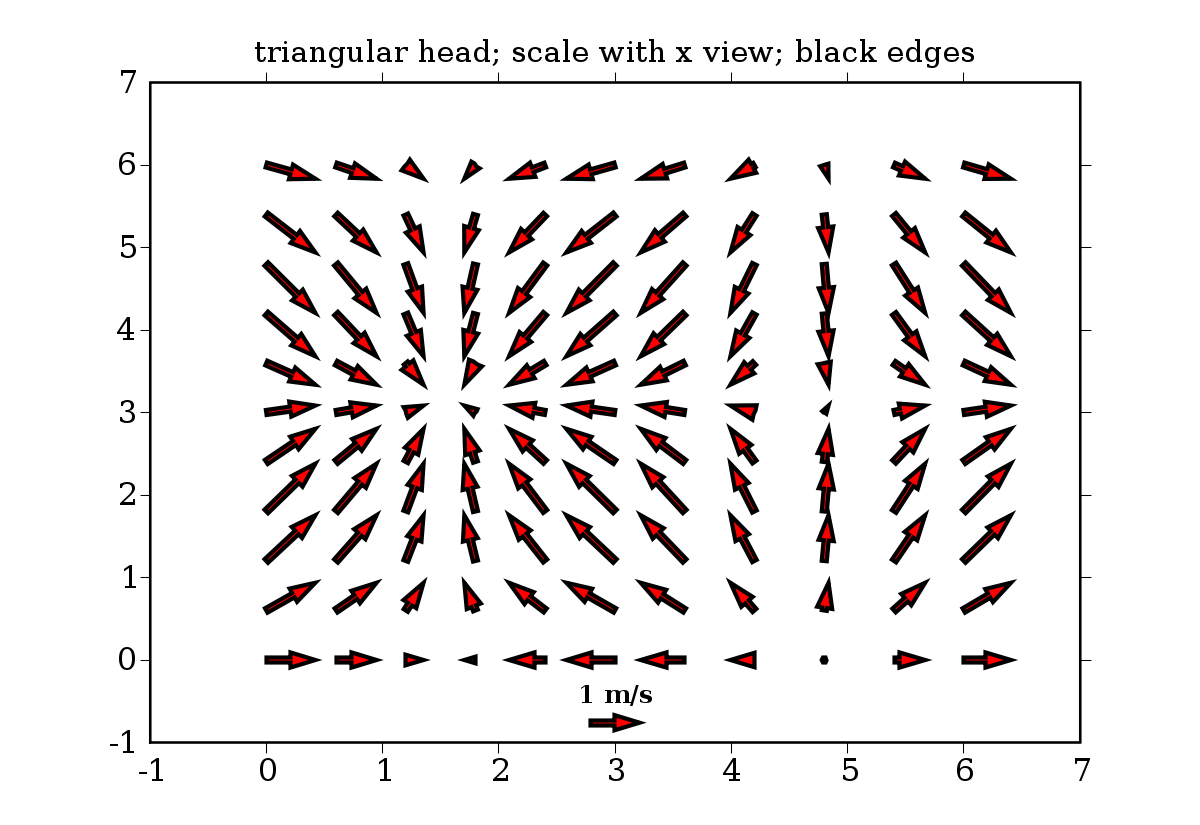
\includegraphics[height=2in, interpolate=true]{data/quiver}  
    \column{0.45\textwidth}
    \begin{block}{Example code}
    \tiny
\begin{lstlisting}
X,Y = meshgrid(arange(0,2*pi,.2),
               arange(0,2*pi,.2) )
U = cos(X)
V = sin(Y)
Q = quiver(X[::3, ::3], Y[::3, ::3], 
           U[::3, ::3], V[::3, ::3],
           color='r', units='x', 
           linewidths=(2,), 
           edgecolors=('k'), 
           headaxislength=5 )
qk = quiverkey(Q, 0.5, 0.03, 1, '1 m/s', 
               fontproperties=
               {'weight': 'bold'})
axis([-1, 7, -1, 7])
title('triangular head; scale '\
      'with x view; black edges')
\end{lstlisting}
  \end{block}
\end{columns}
\end{frame}

\begin{frame}[fragile] \frametitle{Maps}
  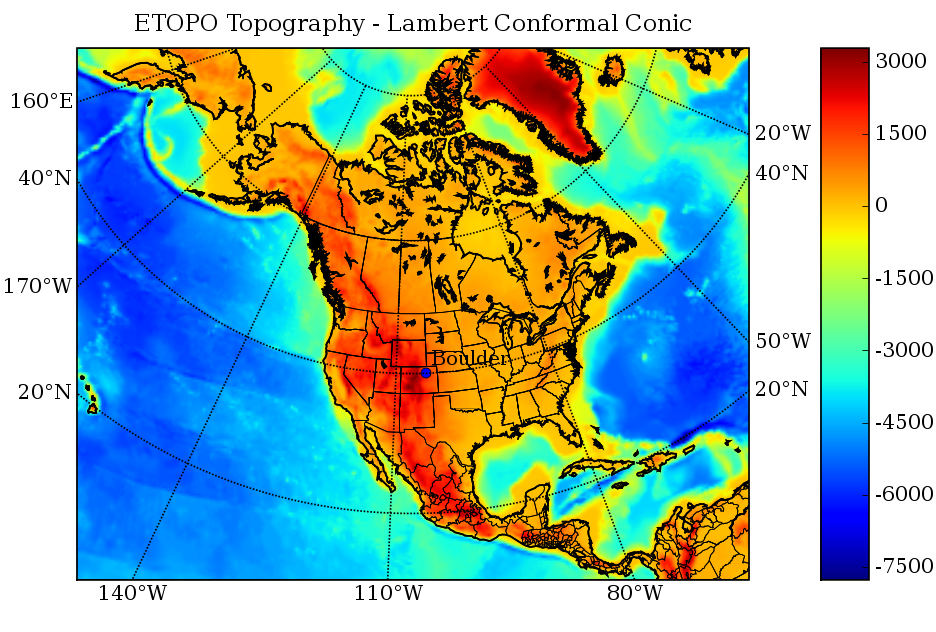
\includegraphics[height=2.5in, interpolate=true]{data/plotmap}  
  \begin{center}
    \tiny
    For details see \url{http://matplotlib.sourceforge.net/screenshots/plotmap.py}
  \end{center}
\end{frame}


\begin{frame}
  \frametitle{More information}
  \begin{itemize}
  \item More information here: \url{http://matplotlib.sf.net}
  \item \url{http://matplotlib.sf.net/tutorial.html}
  \item \url{http://matplotlib.sf.net/screenshots.html}
  \end{itemize}

  \inctime{25}
\end{frame}

\begin{frame}
  \frametitle{Problem set 1.0}
  \begin{enumerate}
      \item Write a function that plots any n-gon given \typ{n}.
      \item Consider the logistic map, $f(x) = kx(1-x)$, plot it for
          $k=2.5, 3.5$ and $4$
\end{enumerate}
\end{frame}

\begin{frame}
  \frametitle{Problem set 1.1}
  \begin{enumerate}
      \item Consider the iteration $x_{n+1} = f(x_n)$ where $f(x) =
          kx(1-x)$.  Plot the successive iterates of this process.
      \item Plot this using a cobweb plot as follows:
          \begin{enumerate}
              \item Start at $(x_0, 0)$
              \item Draw line to $(x_i, f(x_i))$; 
              \item Set $x_{i+1} = f(x_i)$
              \item Draw line to $(x_i, x_i)$
              \item Repeat from 2 for as long as you want 
          \end{enumerate}
    \end{enumerate}
\end{frame}

\begin{frame}
  \frametitle{Problem set 1.2}
  \begin{enumerate}

      \item Plot the Koch snowflake.  Write a function to generate the
          necessary points given the two points constituting a line.
          \pause
          \begin{enumerate}
              \item Split the line into 4 segments.
              \item The first and last segments are trivial.
              \item To rotate the point you can use complex numbers,
                  recall that $z e^{j \theta}$ rotates a point $z$ in 2D
                  by $\theta$.
              \item Do this for all line segments till everything is
                  done.
          \end{enumerate}
      \item Show rate of convergence for a first and second order finite
          difference of sin(x)
\end{enumerate}
\inctime{30}
\end{frame}


%%%%%%%%%%%%%%%%%%%%%%%%%%%%%%%%%%%%%%%%%%%%%%%%%%%%%%%%%%%%%%%%%%%%%%%%%%%%%%%%

\begin{frame}[fragile]
  \frametitle{More IPython features}
  \begin{itemize}
  \item Input and output caching:
    \begin{itemize}
    \item \verb+In+: a list of all entered input
    \item \verb+Out+: a dict of all output
    \item \verb+%hist [-n]+ macro shows previous history, \verb+-n+
      suppresses line number information
    \end{itemize}
  \item Log the session using \verb+%logstart+, \verb+%logon+ and
    \verb+%logoff+
  \item Use \verb+;+ to suppress printing output
  \item \verb+%time statement+
  \item \verb+%timeit [-n<N> -r<R> [-t|-c]] statement+

  \end{itemize}
\end{frame}

\begin{frame}[fragile]
  \frametitle{More IPython features}
  \begin{itemize}
  \item \verb+%run [options] file[.py]+ -- running Python code
  \item \verb+%prun+ runs a statement/expression under the profiler
  \item \verb+%debug+: Helps with debugging after a crash
  \end{itemize}
\end{frame}

\begin{frame}[fragile]
  \frametitle{More IPython features \ldots}
  \begin{itemize}
  \item \verb+%edit [options] [args]+: edit lines of code or file
    specified in editor (configure editor via \verb+$EDITOR+)
  \item \verb+%cd+ changes directory, see also \verb+%pushd, %popd, %dhist+
  \item Shell access
    \begin{itemize}
    \item \verb+!command+ runs a shell command and returns its output
    \item \verb+files = !ls+ sets
      \verb+files+ to all result of the \verb+ls+ command
    \item \verb+!ls $files+ passes the \verb+files+ variable to the
      shell command
  \end{itemize}
    \end{itemize}
\end{frame}

\begin{frame}[fragile]
  \frametitle{More IPython features \ldots}
  \begin{itemize}
  \item \verb+%bookmark+: store a bookmarked location, for use with \verb+%cd+
  \item \verb+%save [options] filename n1-n2 n3-n4+: save lines to a
    file
  \item Can define and use profiles to setup IPython differently:
    \verb+math, scipy, numeric, pysh+ etc.
  \item \verb+%magic+: \alert{Show help on all magics}
  \item Check out the \verb+%macro+ magic
  \end{itemize}
\end{frame}

\begin{frame}
  \frametitle{Problem set 2}
  \begin{itemize}
    \item Compare your linspace with that of numpy for 1 million
        elements in terms of speed.
\end{itemize}
\inctime{10}
\end{frame}


\begin{frame}[fragile]
    \frametitle{Debugging effectively}

    \begin{itemize}
        \item  \kwrd{print} based strategy
        \item Process: Hypothesis, test, refine, rinse-repeat
        \item Using \typ{\%debug} and \typ{\%pdb} in IPython
    \end{itemize}

    \inctime{10} 
\end{frame}

\section{Debugging and testing}

\begin{frame}[fragile]
    \frametitle{Testing code with \typ{nosetests}}
   
    \begin{itemize}
        \item Writing tests is really simple!

        \item Using nose

        \item Example!
    \end{itemize}
\end{frame}

\begin{frame}[fragile]
    \frametitle{Nosetest}
\begin{lstlisting}
def gcd(a, b):
    """Returns gcd of a and b, 
     handles only positive numbers."""
    if a%b == 0: return b
    return gcd(b, a%b)
def lcm(a, b):
    return a*b/gcd(a, b)

if __name__ == '__main__':
    import nose
    nose.main()
\end{lstlisting}

    \inctime{10} 
\end{frame}

\section{NumPy and SciPy}

\begin{frame}
    {More Numpy}

    \begin{itemize}
        \item Multi-dimensional arrays
        \item Random number generation
    \end{itemize}

\end{frame}

\begin{frame}[fragile]
  \frametitle{Multi-dimensional arrays}
\begin{lstlisting}
>>> a = array([[ 0, 1, 2, 3],
...            [10,11,12,13]])
>>> a.shape # (rows, columns)
(2, 4)
# Accessing and setting values
>>> a[1,3] 
13
>>> a[1,3] = -1
>>> a[1] # The second row
array([10,11,12,-1])

\end{lstlisting}
\end{frame}

\begin{frame}[fragile]
  \frametitle{Slicing arrays}
\begin{lstlisting}
>>> a = array([[1,2,3], [4,5,6], 
               [7,8,9]])
>>> a[0,1:3]
array([2, 3])
>>> a[1:,1:]
array([[5, 6],
       [8, 9]])
>>> a[:,2]
array([3, 6, 9])
\end{lstlisting}
\end{frame}
\begin{frame}[fragile]
  \frametitle{Striding arrays}
\begin{lstlisting}
>>> a[0::2,0::2]
array([[1, 3],
       [7, 9]])
# Slices are references to the 
# same memory!
\end{lstlisting}
\end{frame}

\begin{frame}[fragile]
  \frametitle{Array creation functions}
  \begin{itemize}
  \item \typ{array(object, dtype=None, \ldots)}
  \item \typ{arange(start, stop=None, step=1 \ldots)}
  \item \typ{linspace(start, stop, num=50, \ldots)}
  \item \typ{ones(shape, dtype=None, \ldots)}
  \item \typ{zeros(shape, dtype=float,\ldots)}
  \item \typ{identity(n)}
  \item \typ{empty(shape, dtype=float,\ldots)}
  \item \typ{ones\_like(x)}, 
  \item \typ{zeros\_like(x)}, \typ{empty\_like(x)}
  \end{itemize}
\end{frame}

\begin{frame}[fragile]
  \frametitle{Array math}
  \begin{itemize}
  \item Basic \alert{elementwise} math (given two arrays \typ{a, b}):
      \typ{+, -, *, /, \%}
  \item Inplace operators: \typ{a += b}, or \typ{add(a, b,
      a)} etc.
  \item Logical operations: \typ{equal (==)}, \typ{not\_equal (!=)},
    \typ{less (<)}, \typ{greater (>)} etc.
  \item Trig and other functions: \typ{sin(x), arcsin(x), sinh(x),
      exp(x), sqrt(x)} etc.
  \item \typ{sum(x, axis=0), product(x, axis=0)} 
  \item \typ{dot(a, b)}
  \end{itemize}
\end{frame}

\begin{frame}[fragile]
  \frametitle{Advanced}
  \begin{itemize}
  \item Only scratched the surface of \num
  \item Ufunc methods: \typ{reduce, accumulate, outer, reduceat}
  \item Typecasting
  \item More functions: \typ{take, choose, where, compress,
      concatenate}
  \item Array broadcasting and \typ{None}
  \end{itemize}
  \inctime{15}
\end{frame}

\begin{frame}
    {Intro to SciPy}
  \begin{itemize}
  \item \url{http://www.scipy.org}
  \item Open source scientific libraries for Python
  \item Based on NumPy
    \end{itemize}

    \inctime{25}
\end{frame}

\begin{frame}
  \frametitle{SciPy}
  \begin{itemize}
  \item Provides:
    \begin{itemize}
    \item Linear algebra
    \item Numerical integration
    \item Fourier transforms
    \item Signal processing
    \item Special functions
    \item Statistics
    \item Optimization
    \item Image processing
    \item ODE solvers
    \end{itemize}
  \item Uses LAPACK, QUADPACK, ODEPACK, FFTPACK etc. from netlib
  \end{itemize}
\end{frame}


\section{3D Plotting}

\begin{frame}
  \frametitle{Introduction to Mayavi}
  \begin{itemize}
  \item Most scientists not interested in details of visualization
  \item Visualization of data files with a nice UI
  \item Interactive visualization of data (think Matlab)
  \item Embedding visualizations in applications
  \item Customization
  \end{itemize}
  \pause
  \begin{block}{The Goal}
      Provide a \alert{flexible} library/app for every one of these needs!
  \end{block}
\end{frame}

\begin{frame}[fragile]
    \frametitle{\typ{mlab}}
  \begin{columns}
    \column{0.62\textwidth}
    \hspace*{-0.45in}
      \footnotesize
\begin{lstlisting}
from enthought.mayavi import mlab
from numpy import ogrid, sin

x, y, z = ogrid[-10:10:100j, 
                -10:10:100j, 
                -10:10:100j]

mlab.contour3d(sin(x*y*z)/(x*y*z))
mlab.show()
\end{lstlisting}
    \column{0.4\textwidth}
    \hspace*{-0.1\linewidth}
    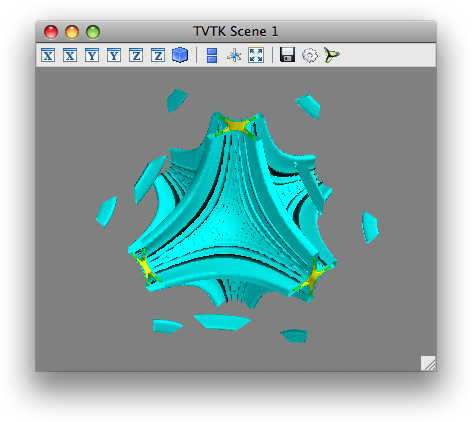
\includegraphics[width=1.18\linewidth]{data/mlab.png}
  \end{columns}
\end{frame}

\begin{frame}
    {A Look at the docs }

    \inctime{20}
\end{frame}


\section{Integration demo: Lorenz equations}

\begin{frame}
    \frametitle{Lorenz equation example}
    \begin{eqnarray*}
        \frac{d x}{dt} &=& s (y-x)\\
        \frac{d y}{d t} &=& rx -y -xz\\
        \frac{d z}{d t} &=& xy - bz\\
    \end{eqnarray*}
    \begin{itemize}
        \item Specifies the evolution of the system
        \item Think: Velocity of a particle in 3D
        \item Lets trace its path
    \end{itemize}
\end{frame}

\begin{frame}
    {Interactive exploration}

    \inctime{25}
\end{frame}


\end{document}

- Numpy arrays (30 mins)
    - Matrices
    - random number generation.
    - Image manipulation: jigsaw puzzle.
    - Monte-carlo integration.





\begin{frame}[fragile]
  \frametitle{More on functions}
  \begin{itemize}
  \item Support default and keyword arguments
  \item Scope of variables in the function is local
  \item Mutable items are \alert{passed by reference}
  \item First line after definition may be a documentation string
    (\alert{recommended!})
  \item Function definition and execution defines a name bound to the
    function
  \item You \emph{can} assign a variable to a function!
  \end{itemize}
\end{frame}


\begin{frame}[fragile]
  \frametitle{Functions: default arguments}
  \begin{lstlisting}
def ask_ok(prompt, retries=4, complaint='Yes or no!'):
    while True:
        ok = raw_input(prompt)
        if ok in ('y', 'ye', 'yes'): 
            return True
        if ok in ('n', 'no', 'nop', 'nope'): 
            return False
        retries = retries - 1
        if retries < 0: 
            raise IOError, 'bad user'
        print complaint
  \end{lstlisting}
\end{frame}

\begin{frame}[fragile]
  \frametitle{Functions: keyword arguments}
  \begin{lstlisting}
def parrot(voltage, state='a stiff', 
           action='voom', type='Norwegian Blue'):
    print "-- This parrot wouldn't", action,
    print "if you put", voltage, "Volts through it."
    print "-- Lovely plumage, the", type
    print "-- It's", state, "!"

parrot(1000)
parrot(action = 'VOOOOOM', voltage = 1000000)
parrot('a thousand', state = 'pushing up the daisies')
parrot('a million', 'bereft of life', 'jump')
\end{lstlisting}
\end{frame}

\begin{frame}[fragile]
  \frametitle{Functions: arbitrary argument lists}
  \begin{itemize}
  \item Arbitrary number of arguments using \verb+*args+ or
    \verb+*whatever+
  \item Keyword arguments using \verb+**kw+
  \item Given a tuple/dict how do you call a function?
    \begin{itemize}
    \item Using argument unpacking
    \item For positional arguments: \verb+foo(*[5, 10])+
    \item For keyword args: \verb+foo(**{'a':5, 'b':10})+
    \end{itemize}
  \end{itemize}
\begin{lstlisting}
def foo(a=10, b=100):
    print a, b
def func(*args, **keyword):
    print args, keyword
# Unpacking:
args = [5, 10]
foo(*args)
kw = {'a':5, 'b':10}
foo(**kw)
\end{lstlisting}
\end{frame}

\subsection{Modules, exceptions, classes}

\begin{frame}
  \frametitle{Modules}
  \begin{itemize}
  \item Define variables, functions and classes in a file with a
    \typ{.py} extension
  \item This file becomes a module!
  \item Modules are searched in the following:
    \begin{itemize}
    \item Current directory
    \item Standard: \typ{/usr/lib/python2.3/site-packages/} etc.
    \item Directories specified in PYTHONPATH
    \item \typ{sys.path}: current path settings (from the \typ{sys}
      module)
    \end{itemize}
  \item The \typ{import} keyword ``loads'' a module
  \item One can also use:
    \mbox{\typ{from module import name1, name2, name2}}\\
    where \typ{name1} etc. are names in the module, ``module''
  \item \typ{from module import *} \ --- imports everything from module,
    \alert{use only in interactive mode}
  \end{itemize}
\end{frame}

\begin{frame}[fragile]
  \frametitle{Modules: example}
  \begin{lstlisting}
# --- foo.py ---
some_var = 1
def fib(n): # write Fibonacci series up to n
    """Print a Fibonacci series up to n."""
    a, b = 0, 1
    while b < n:
        print b,
        a, b = b, a+b
# EOF

>>> import foo
>>> foo.fib(10)
1 1 2 3 5 8 
>>> foo.some_var
1
  \end{lstlisting}
\end{frame}

\begin{frame}[fragile]
  \frametitle{Namespaces}
  \begin{itemize}
  \item A mapping from names to objects
  \item Modules introduce a namespace 
  \item So do classes
  \item The running script's namespace is \verb+__main__+
  \item A modules namespace is identified by its name
  \item The standard functions (like \typ{len}) are in the
    \verb+__builtin__+ namespace
  \item Namespaces help organize different names and their bindings to
    different objects
  \end{itemize}
\end{frame}

\begin{frame}
  \frametitle{Exceptions}
  \begin{itemize}
  \item Python's way of notifying you of errors
  \item Several standard exceptions: \typ{SyntaxError}, \typ{IOError}
    etc.
  \item Users can also \typ{raise} errors
  \item Users can create their own exceptions
  \item Exceptions can be ``caught'' via \typ{try/except} blocks
  \end{itemize}
\end{frame}

\begin{frame}[fragile]
  \frametitle{Exception: examples}
\begin{lstlisting}
>>> 10 * (1/0)
Traceback (most recent call last):
  File "<stdin>", line 1, in ?
ZeroDivisionError: integer division or modulo by zero
>>> 4 + spam*3
Traceback (most recent call last):
  File "<stdin>", line 1, in ?
NameError: name 'spam' is not defined
>>> '2' + 2
Traceback (most recent call last):
  File "<stdin>", line 1, in ?
TypeError: cannot concatenate 'str' and 'int' objects
\end{lstlisting}
\end{frame}

\begin{frame}[fragile]
  \frametitle{Exception: examples}
\begin{lstlisting}
>>> while True:
...     try:
...         x = int(raw_input("Enter a number: "))
...         break
...     except ValueError:
...         print "Invalid number, try again..."
...
>>> # To raise exceptions
... raise ValueError, "your error message"
Traceback (most recent call last):
  File "<stdin>", line 2, in ?
ValueError: your error message
\end{lstlisting}
\end{frame}

\begin{frame}[fragile]
  \frametitle{Classes: the big picture}
  \begin{itemize}
  \item Lets you create new data types
  \item Class is a template for an object belonging to that class
  \item Note: in Python a class is also an object
  \item Instantiating a class creates an instance (an object)
  \item An instance encapsulates the state (data) and behavior
    (methods)
  \item Allows you to define an inheritance hierarchy
    \begin{itemize}
    \item ``A Honda car \alert{is a} car.''
    \item ``A car \alert{is an} automobile.''
    \item ``A Python \alert{is a} reptile.''
    \end{itemize}
  \item Programmers need to think OO
  \end{itemize}
\end{frame}

\begin{frame}[fragile]
  \frametitle{Classes: what's the big deal?}
  \begin{itemize}
  \item Lets you create objects that mimic a real problem being
    simulated
  \item Makes problem solving more natural and elegant
  \item Easier to create code
  \item Allows for code-reuse
  \item Polymorphism
  \end{itemize}
\end{frame}

\begin{frame}[fragile]
  \frametitle{Class definition and instantiation}
  \begin{itemize}
  \item Class definitions when executed create class objects
  \item Instantiating the class object creates an instance of the
    class
  \end{itemize}
\footnotesize
\begin{lstlisting}
class Foo(object):
    pass
# class object created.
# Create an instance of Foo.
f = Foo()
# Can assign an attribute to the instance
f.a = 100
print f.a
100
\end{lstlisting}
\end{frame}

\begin{frame}[fragile]
  \frametitle{Classes \ldots}
  \begin{itemize}
  \item All attributes are accessed via the \typ{object.attribute}
    syntax
  \item Both class and instance attributes are supported
  \item \emph{Methods} represent the behavior of an object: crudely
    think of them as functions ``belonging'' to the object
  \item All methods in Python are ``virtual''
  \item Inheritance through subclassing
  \item Multiple inheritance is supported
  \item No special public and private attributes: only good
    conventions
    \begin{itemize}
    \item \verb+object.public()+: public
    \item \verb+object._private()+ \& \verb+object.__priv()+: 
      non-public
    \end{itemize}
  \end{itemize}
\end{frame}

\begin{frame}[fragile]
  \frametitle{Classes: examples}
\begin{lstlisting}
class MyClass(object):
    """Example class (this is the class docstring)."""
    i = 12345 # A class attribute
    def f(self):
        """This is the method docstring"""
        return 'hello world'

>>> a = MyClass() # creates an instance
>>> a.f()
'hello world'
>>> # a.f() is equivalent to MyClass.f(a)
... # This also explains why f has a 'self' argument.
... MyClass.f(a)
'hello world'
\end{lstlisting}
\end{frame}

\begin{frame}[fragile]
  \frametitle{Classes (continued)}
  \begin{itemize}
  \item \typ{self} is \alert{conventionally} the first argument for a
    method
  \item In previous example, \typ{a.f} is a method object
  \item When \typ{a.f} is called, it is passed the instance \typ{a} as
    the first argument
  \item If a method called \verb+__init__+ exists, it is called when
    the object is created
  \item If a method called \verb+__del__+ exists, it is called before
    the object is garbage collected
  \item Instance attributes are set by simply ``setting'' them in
    \typ{self}
  \item Other special methods (by convention) like \verb+__add__+ let
    you define numeric types:
    {\footnotesize \url{http://docs.python.org/ref/specialnames.html}
      \\ \url{http://docs.python.org/ref/numeric-types.html}
    }
  \end{itemize}
\end{frame}

\begin{frame}[fragile]
  \frametitle{Classes: examples}
\begin{lstlisting}
class Bag(MyClass): # Shows how to derive classes
    def __init__(self): # called on object creation.
        self.data = [] # an instance attribute
    def add(self, x):
        self.data.append(x)
    def addtwice(self, x):
        self.add(x)
        self.add(x)
>>> a = Bag()
>>> a.f() # Inherited method
'hello world'
>>> a.add(1); a.addtwice(2)
>>> a.data
[1, 2, 2]
\end{lstlisting}
\end{frame}

\begin{frame}[fragile]
  \frametitle{Derived classes}
  \begin{itemize}
  \item Call the parent's \verb+__init__+ if needed
  \item If you don't need a new constructor, no need to define it in subclass
  \item Can also use the \verb+super+ built-in function
  \end{itemize}
\begin{lstlisting}
class AnotherBag(Bag):
    def __init__(self):
        # Must call parent's __init__ explicitly
        Bag.__init__(self)
        # Alternatively use this:
        super(AnotherBag, self).__init__()
        # Now setup any more data.
        self.more_data = []
\end{lstlisting}
\end{frame}

\begin{frame}[fragile]
  \frametitle{Classes: polymorphism}
\begin{lstlisting}
class Drawable(object):
    def draw(self):
        # Just a specification.
        pass
\end{lstlisting}
\mode<presentation>{\pause}
\begin{lstlisting}
class Square(Drawable):
    def draw(self):
        # draw a square.
class Circle(Drawable):
    def draw(self):
        # draw a circle.
\end{lstlisting}
\mode<presentation>{\pause}
\begin{lstlisting}
class Artist(Drawable):
    def draw(self):
        for obj in self.drawables:
            obj.draw()
\end{lstlisting}
\end{frame}

\subsection{Miscellaneous}

\begin{frame}[fragile]
  \frametitle{Stand-alone scripts}
Consider a file \typ{f.py}:
\begin{lstlisting}
#!/usr/bin/env python
"""Module level documentation."""
# First line tells the shell that it should use Python
# to interpret the code in the file.
def f():
    print "f"

# Check if we are running standalone or as module.
# When imported, __name__ will not be '__main__'
if __name__ == '__main__':
    # This is not executed when f.py is imported.
    f() 
\end{lstlisting}
\end{frame}

\begin{frame}[fragile]
  \frametitle{List comprehensions}
\begin{lstlisting}
>>> veg = ['tomato', 'cabbage', 'carrot', 'potato']
>>> [x.upper() for x in veg]
['TOMATO', 'CABBAGE', 'CARROT', 'POTATO']
>>> vec = range(0, 8)
>>> even = [x for x in vec if x%2 == 0]
>>> even
[0, 2, 4, 6]
>>> [x*x for x in even]
[0, 4, 16, 36]
>>> odd = [x for x in vec if x%2 == 1]
>>> odd
[1, 3, 5, 7]
>>> [x*y for x in even for y in odd]
[0, 0, 0, 0, 2, 6, 10, 14, 4, 12, 20, 28, 6, 18,30,42]
\end{lstlisting}
\end{frame}

\begin{frame}[fragile]
  \frametitle{File handling}
\begin{lstlisting}
>>> # Reading files:
... f = open('/path/to/file_name')
>>> data = f.read() # Read entire file.
>>> line = f.readline() # Read one line.
>>> # Read entire file appending each line into a list
... lines = f.readlines()
>>> f.close() # close the file.
>>> # Writing files:
... f = open('/path/to/file_name', 'w')
>>> f.write('hello world\n')
\end{lstlisting}
  \begin{itemize}
  \item \typ{tell()}: returns int of current position
  \item \typ{seek(pos)}: moves current position to specified byte
  \item Call \typ{close()} when done using a file
  \end{itemize}
\end{frame}

\begin{frame}[fragile]
  \frametitle{Math}
  \begin{itemize}
  \item \typ{math} module provides basic math routines for
    floats
  \item \typ{cmath} module provides math routies for complex
    numbers
  \item \typ{random}: provides pseudo-random number generators
    for various distributions
  \item These are always available and part of the standard library
  \item More serious math is provided by the NumPy/SciPy modules --
    these are not standard and need to be installed separately
  \end{itemize}
\end{frame}

\begin{frame}[fragile]
  \frametitle{Timing and profiling}
  \begin{itemize}
  \item Timing code: use the \typ{time} module
  \item Read up on \typ{time.time()} and \typ{time.clock()}
  \item \typ{timeit}: is a better way of doing timing
  \item IPython has handy \typ{time} and \typ{timeit} macros (type
    \typ{timeit?} for help)
  \item IPython lets you debug and profile code via the \typ{run}
    macro (type \typ{run?} on the prompt to learn more)
  \end{itemize}
\end{frame}

\begin{frame}[fragile]
  \frametitle{Odds and ends}
  \begin{itemize}
  \item \typ{dir([object])} function: attributes of given object
  \item \typ{type(object)}: returns type information
  \item \typ{str(), repr()}: convert object to string representation
  \item \typ{isinstance, issubclass}
  \item \typ{assert} statements let you do debugging assertions in
    code
  \item \typ{csv} module: reading and writing CSV files
  \item \typ{pickle}: lets you save and load Python objects
    (\alert{serialization})
  \item \typ{sys.argv}: command line arguments
  \item \typ{os.path}: common path manipulations
  \item Check out the Python Library reference:
    \url{http://docs.python.org/lib/lib.html}
  \end{itemize}
\end{frame}

\begin{frame}[fragile]
  \frametitle{Test driven development (TDD)}
  \begin{itemize}
      \item Why?
          \begin{itemize}

            \item Forces you to write reusable code!

            \item Think about the API

            \item More robust

            \item Makes refactoring very easy

          \end{itemize}
      \item How?  Python offers three major ways of doing this
          \begin{itemize}
              \item doctest
              \item unittest
              \item nosetest (and similar like py.test)
          \end{itemize}

      \item Test every piece of functionality you offer

      \item This isn't a formal introduction but more a practical one

  \end{itemize}
\end{frame}

\begin{frame}[fragile]
  \frametitle{Unit test}
\begin{lstlisting}
import unittest

class MyTestCase(unittest.TestCase):
    def setUp(self):
        # Called *before* each test_* 
    def tearDown(self):
        # Called *after* each test_* 
    def test_something(self):
        "docstring"
        #  Test code.
        self.assertEqual(x, y)
        self.assertRaises(ValueError, func, arg1, arg2 ...)

if __name__ == '__main__':
    unittest.main() 
\end{lstlisting}
\end{frame}

\begin{frame}[fragile]
    \frametitle{Nosetest}
\begin{lstlisting}
import particle
def test_particle():
    # Use asserts here.
    p = particle.Particle(1.0)
    assert p.property[0] == 1.0
    assert p.property[2] == 0.0

if __name__ == '__main__':
    import nose
    nose.main()
\end{lstlisting}
\end{frame}

\begin{frame}[fragile]
  \frametitle{Testing}
  \begin{itemize}
      \item More details: see library reference and search for nosetest
  \end{itemize}
\end{frame}

\section{Numerics \& Plotting}

\subsection{NumPy Arrays}

\subsection{Plotting: Matplotlib}

\begin{frame}
  \frametitle{About \texttt{matplotlib}}
  \begin{itemize}
  \item Easy to use, scriptable, ``Matlab-like'' 2D plotting
  \item Publication quality figures and interactive capabilities
  \item Plots, histograms, power spectra, bar charts, errorcharts,
    scatterplots, etc.
  \item Also does polar plots, maps, contours
  \item Support for simple \TeX\ markup
  \item Multiple output backends (images, EPS, SVG, wx, Agg, Tk, GTK)
  \item Cross-platform: Linux, Win32, Mac OS X
  \item Good idea to use via IPython:  \typ{ipython -pylab}
  \item From scripts use: \typ{import pylab}
  \end{itemize}
\end{frame}

\begin{frame}
  \frametitle{More information}
  \begin{itemize}
  \item More information here: \url{http://matplotlib.sf.net}
  \item \url{http://matplotlib.sf.net/tutorial.html}
  \item \url{http://matplotlib.sf.net/screenshots.html}
  \end{itemize}
\end{frame}

\begin{frame}[fragile]
  \frametitle{Basic plotting with \texttt{matplotlib}}
\begin{lstlisting}
>>> x = arange(0, 2*pi, 0.05)
>>> plot(x, sin(x)) # Same as plot(x, sin(x), 'b-') 
>>> plot(x, sin(x), 'ro')
>>> axis([0,2*pi, -1,1])
>>> xlabel(r'$\chi$', color='g')
>>> ylabel(r'sin($\chi$)', color='r')
>>> title('A simple figure', fontsize=20)
>>> savefig('/tmp/test.eps')
# Multiple plots in one figure
>>> t = arange(0.0, 5.2, 0.2)
# red dashes, blue squares and green triangles
>>> plot(t, t, 'r--', t, t**2, 'bs', t, t**3, 'g^')
\end{lstlisting}
\end{frame}

\begin{frame}[fragile]
  \frametitle{Basic plotting \ldots}
\begin{lstlisting}
# Set properties of objects:
>>> plot(x, sin(x), linewidth=2.0, color='r')
>>> l, = plot(x, sin(x))
>>> setp(l, linewidth=2.0, color='r')
>>> l.set_linewidth(2.0); l.set_color('r')
>>> draw() # Redraws current figure.
>>> setp(l) # Prints available properties
>>> close() # Closes the figure.
# Multiple figures:
>>> figure(1); plot(x, sin(x))
>>> figure(2); plot(x, tanh(x))
>>> figure(1); title('Easy as 1,2,3')
\end{lstlisting}
\end{frame}

\begin{frame}[fragile]
  \frametitle{Basic plotting \ldots}
\begin{lstlisting}
>>> figure(1)
>>> subplot(211) # Same as subplot(2, 1, 1)
>>> plot(x, cos(5*x)*exp(-x))
>>> subplot(2, 1, 2)
>>> plot(x, cos(5*x), 'r--', label='cosine')
>>> plot(x, sin(5*x), 'g--', label='sine')
>>> legend() # Or legend(['cosine', 'sine'])
>>> text(1,0, '(1,0)')
>>> axes = gca() # Current axis
>>> fig = gcf() # Current figure
\end{lstlisting}
\end{frame}


\subsection{SciPy}

\begin{frame}
  \frametitle{Using \texttt{SciPy}}
  \begin{itemize}
  \item SciPy is Open Source software for mathematics, science, and
    engineering
  \item \typ{import scipy}
  \item Built on NumPy
  \item Provides modules for statistics, optimization, integration,
    linear algebra, Fourier transforms, signal and image processing,
    genetic algorithms, ODE solvers, special functions, and more
  \item Used widely by scientists world over
  \item Details are beyond the scope of this tutorial
  \end{itemize}
\end{frame}

\section{Standard library}

\subsection{Quick Tour}

\begin{frame}
  \frametitle{Standard library}
  \begin{itemize}
  \item Very powerful
  \item ``Batteries included''
  \item Example standard modules taken from the tutorial
    \begin{itemize}
    \item Operating system interface: \typ{os}
    \item System, Command line arguments: \typ{sys}
    \item Regular expressions: \typ{re}
    \item Math: \typ{math}, \typ{random}
    \item Internet access: \typ{urllib2}, \typ{smtplib}
    \item Data compression: \typ{zlib}, \typ{gzip}, \typ{bz2},
      \typ{zipfile}, and \typ{tarfile}
    \item Unit testing: \typ{doctest} and \typ{unittest}
    \item And a whole lot more!
    \end{itemize}
  \item Check out the Python Library reference:
    \url{http://docs.python.org/lib/lib.html}
  \end{itemize}
\end{frame}

\begin{frame}[fragile]
  \frametitle{Stdlib: examples}
\begin{lstlisting}
>>> import os
>>> os.system('date')
Fri Jun 10 22:13:09 IST 2005
0
>>> os.getcwd()
'/home/prabhu'
>>> os.chdir('/tmp')
>>> import os
>>> dir(os)
<returns a list of all module functions>
>>> help(os)
<extensive manual page from module's docstrings>
\end{lstlisting}
\end{frame}

\begin{frame}[fragile]
  \frametitle{Stdlib: examples}
\begin{lstlisting}
>>> import sys
>>> # Print the list of command line args to Python
... print sys.argv 
['']
>>> import re # Regular expressions
>>> re.findall(r'\bf[a-z]*', 
... 'which foot or hand fell fastest')
['foot', 'fell', 'fastest']
>>> re.sub(r'(\b[a-z]+) \1', r'\1', 
... 'cat in the the hat')
'cat in the hat'
\end{lstlisting}
\end{frame}

\begin{frame}[fragile]
  \frametitle{Stdlib: examples}
\begin{lstlisting}
>>> import math
>>> math.cos(math.pi / 4.0)
0.70710678118654757
>>> math.log(1024, 2)
10.0
>>> import random
>>> random.choice(['apple', 'pear', 'banana'])
'pear'
\end{lstlisting}
\end{frame}

\begin{frame}[fragile]
  \frametitle{Stdlib: examples}
\begin{lstlisting}
>>> import urllib2
>>> f = urllib2.urlopen('http://www.python.org/')
>>> print f.read(100)
<!DOCTYPE html PUBLIC "-//W3C//DTD HTML 4.01 Transitional//EN">
<?xml-stylesheet href="./css/ht2html
\end{lstlisting}
\end{frame}

\begin{frame}[fragile]
  \frametitle{Stdlib: examples}
\begin{lstlisting}
>>> import zlib
>>> s = 'witch which has which witches wrist watch'
>>> len(s)
41
>>> t = zlib.compress(s)
>>> len(t)
37
>>> zlib.decompress(t)
'witch which has which witches wrist watch'
>>> zlib.crc32(t)
-1438085031
\end{lstlisting}
\end{frame}

\begin{frame}
  \frametitle{Summary}
  \begin{itemize}
  \item Introduced Python
  \item Basic syntax
  \item Basic types and data structures
  \item Control flow
  \item Functions
  \item Modules
  \item Exceptions
  \item Classes
  \item Standard library
  \end{itemize}
\end{frame}

\end{document}

\subsection{Basic data structures}
\begin{frame}{Lists}
  \begin{itemize}
    \item \texttt{species = [ 'humans', 'orcs', 'elves', 'dwarves' ]}
    \item \texttt{ ids = [ 107, 109, 124, 141, 142, 144 ]}
    \item \texttt{ oneliners = [ 'I will be back', 'Do or do not! No try!!', 42 ] }
  \end{itemize}

  \begin{block}{List operations}
    ids + [ 100, 102 ]\\
    species.append( 'unicorns')\\
    print oneliners[ 1 ]\\
    look up \alert{docs.python.org/tutorial/datastructures.html}
  \end{block}
\end{frame}
\end{document}
\section{Python Tutorial}
\subsection{Preliminaries}
\begin{frame}
  \frametitle{Using the interpreter}
  \begin{itemize}
  \item Starting up: \typ{python} or \typ{ipython}
  \item Quitting: \typ{Control-D} or \typ{Control-Z} (on Win32)
  \item Can use it like a calculator
  \item Can execute one-liners via the \typ{-c} option:
    \typ{python -c "print 'hello world'"}
  \item Other options via \typ{python -h}
  \end{itemize}
\end{frame}

\begin{frame}
  \frametitle{IPython}
  \begin{itemize}
  \item Recommended interpreter, IPython:
    \url{http://ipython.scipy.org}
  \item Better than the default Python shell
  \item Supports tab completion by default
  \item Easier object introspection
  \item Shell access!
  \item Command system to allow extending its own behavior
  \item Supports history (across sessions) and logging
  \item Can be embedded in your own Python code
  \item Support for macros
  \item A flexible framework for your own custom interpreter
  \item Other miscellaneous conveniences
  \item We'll get back to this later
  \end{itemize}
\end{frame}

\begin{frame}[fragile]
  \frametitle{Basic IPython features}
  \begin{itemize}
  \item Startup: \verb+ipython [options] files+
    \begin{itemize}
    \item \verb+ipython [-wthread|-gthread|-qthread]+:
      Threading modes to support wxPython, pyGTK and Qt
    \item \verb+ipython -pylab+: Support for matplotlib
    \end{itemize}
  \item TAB completion:
    \begin{itemize}
    \item Type \verb+object_name.<TAB>+ to see list of options
    \item Also completes on file and directory names
    \end{itemize}
  \item \verb+object?+ shows docstring/help for any Python object
  \item \verb+object??+ presents more docs (and source if possible)
  \item Debugging with \verb+%pdb+ magic: pops up pdb on errors
  \item Access history (saved over earlier sessions also)
    \begin{itemize}
    \item Use \texttt{<UpArrow>}: move up history
    \item Use \texttt{<Ctrl-r> string}: search history backwards
    \item Use \texttt{Esc >}: get back to end of history
    \end{itemize}
  \item \verb+%run [options] file[.py]+ lets you run Python code
  \end{itemize}
\end{frame}
% LocalWords:  BDFL Guido Rossum PSF Nokia OO Zope CMS RedHat SciPy MayaVi spam
% LocalWords:  IPython ipython stdin TypeError dict int elif PYTHONPATH IOError
% LocalWords:  namespace Namespaces SyntaxError ZeroDivisionError NameError str
% LocalWords:  ValueError subclassed def


  \item Types are of two kinds: \alert{mutable} and \alert{immutable}
  \item Immutable types: numbers, strings, \typ{None} and tuples
  \item Immutables cannot be changed ``in-place''
  \item Mutable types: lists, dictionaries, instances, etc.
  \item Mutable objects can be ``changed''
  \end{itemize}


\begin{frame}
  \frametitle{Important!}
  \begin{itemize}
    \item Assignment to an object is by reference
    \item Essentially, \alert{names are bound to objects}
  \end{itemize}
\end{frame}


\end{document}
\begin{frame}[fragile]
  \frametitle{Dictionaries}
  \begin{itemize}
  \item Associative arrays/mappings
  \item Indexed by ``keys'' (keys must be immutable)
  \item \typ{dict[key] = value}
  \item \typ{keys()} returns all keys of the dict
  \item \typ{values()} returns the values of the dict
  \item \verb+has_key(key)+ returns if \typ{key} is in the dict
  \end{itemize}
\end{frame}

\begin{frame}[fragile]
  \frametitle{Dictionaries: example}
  \begin{lstlisting}
>>> tel = {'jack': 4098, 'sape': 4139}
>>> tel['guido'] = 4127
>>> tel
{'sape': 4139, 'guido': 4127, 'jack': 4098}
>>> tel['jack']
4098
>>> del tel['sape']
>>> tel['irv'] = 4127
>>> tel
{'guido': 4127, 'irv': 4127, 'jack': 4098}
>>> tel.keys()
['guido', 'irv', 'jack']
>>> tel.has_key('guido')
True
  \end{lstlisting}
\end{frame}

\subsection{Control flow, functions}



\begin{frame}[fragile]
  \frametitle{\typ{If} example}
  \begin{lstlisting}
>>> a = ['cat', 'window', 'defenestrate']
>>> if 'cat' in a:
...    print "meaw"
...
meaw
>>> pets = {'cat': 1, 'dog':2, 'croc': 10}
>>> if 'croc' in pets:
...    print pets['croc']
...
10
  \end{lstlisting}
\end{frame}

\begin{frame}[fragile]
  \frametitle{\typ{for} example}
  \begin{lstlisting}
>>> a = ['cat', 'window', 'defenestrate']
>>> for x in a:
...     print x, len(x)
...
cat 3
window 6
defenestrate 12
>>> knights = {'gallahad': 'the pure', 
... 'robin': 'the brave'}
>>> for k, v in knights.iteritems():
...     print k, v
...
gallahad the pure
robin the brave
\end{lstlisting}
\end{frame}
